% -*- TeX-engine: xetex -*-

\documentclass[xetex,aspectratio=169,14pt,hyperref={pdfpagelabels=true,pdflang={en-GB}}]{beamer}

\usepackage[sci,noslidestrathidentity]{strathclyde}
\strathsetidentity{Department of}{Computer \& Information Sciences}

\usepackage{lmodern}
\usepackage{subscript}
\usepackage{url}
\usepackage{pifont}
\usepackage{csquotes}
\usepackage{mathpartir}
\usepackage{stmaryrd}
\usepackage{multirow}
\usepackage{euler}
\usepackage[normalem]{ulem}

% 2013-09-08 SU adding xetex specifics
% http://www.woggie.net/2008/07/16/beamer-pdftex-and-xetex/
\usepackage{xltxtra}

% 2013-09-08 SU http://robjhyndman.com/hyndsight/xelatex/
\defaultfontfeatures{Ligatures=TeX}

% 2015-12-09 SU table beautified
\renewcommand{\arraystretch}{1.2}
\usepackage{booktabs}

%MGK compatibility
\newcommand{\hh}[1]
  {\medskip\textbf{\large #1}}
\newcommand{\pdu}[3]
  {#1\rightarrow #2 : &\ & \makebox[70mm][l]{$#3$}}



\setlength{\marginparwidth}{2cm}
\usepackage{todonotes}%[disable]
\let\OldTodo\todo
\renewcommand{\todo}{\OldTodo[inline]}%
\newcommand{\todolater}[1]{}% Things to do for next year


\DeclareTextCommandDefault{\nobreakspace}{\leavevmode\nobreak\ }
\usepackage{rotating}

\usepackage{pdfcomment}% To add alt text for images using \pdftooltip{}

\usepackage{appendixnumberbeamer}

\newcommand{\messageframe}[1]{\begin{frame}\begin{center}\Huge #1\end{center}\end{frame}}
\newcommand{\sechead}[1]{{\bf #1} \\}
\newcommand{\examplehead}[1]{{\bf Example:} {\it\textcolor{red!90}{#1}} \\}
\newcommand{\eqnote}[1]{\hspace{3cm}\textit{#1}}
\newcommand{\sidenote}[1]{\qquad {\footnotesize \textcolor{black!60}{(#1)}}}
\newcommand{\sem}[1]{\llbracket #1 \rrbracket}
\newcommand{\true}{\mathsf{T}}
\newcommand{\false}{\mathsf{F}}

\def\strikeafter<#1>#2{\temporal<#1>{#2}{\sout{#2}}{\sout{#2}}}


%\newcommand{\rhighlight}{\textcolor{titlered}}
\newcommand{\rhighlight}{\textbf}
\newcommand{\highlight}{\textbf}

% \setmainfont{Linux Biolinum O}
\setmainfont{LinBiolinum}[
Path=,
UprightFont = *_R.otf ,
BoldFont = *_RB.otf ,
ItalicFont = *_RI.otf
]

\setbeamertemplate{navigation symbols}{}
%\usecolortheme[rgb={0.8,0,0}]{structure}
\usefonttheme{serif}
\usefonttheme{structurebold}
\setbeamercolor{description item}{fg=black}


\author[Atkey]{Dr.~Robert Atkey}
\institute[Strathclyde]{Computer \& Information Sciences}
\date[]{}

\newcommand{\weeksection}[1]{%
  \section{\thetitle{}, Part~\thesection : #1}
  \begin{frame}
    \begin{center}
      \textcolor{black!60}{\thetitle{}, Part \thesection}\\
      {\Huge #1}
    \end{center}
  \end{frame}}

\newcommand{\weektitle}[2]{\def\thetitle{#2}
\title[CS208 - Week #1]{CS208 (Semester 1) Week #1 : #2}}

\newcommand{\assigned}{:}

\newcommand{\forcedto}{\assigned_f}
\newcommand{\decideto}{\assigned_d}


\weektitle{5}{Natural Deduction II}

\begin{document}

\frame{\titlepage}

\weeksection{Rules for ``Or''}

\begin{frame}
  {``Or'' Introduction}

  \bigskip

  \begin{mathpar}
    \inferrule* [right=Left]
    {\Gamma \vdash Q_1}
    {\Gamma \vdash Q_1 \lor Q_2}

    \inferrule* [right=Right]
    {\Gamma \vdash Q_2}
    {\Gamma \vdash Q_1 \lor Q_2}
  \end{mathpar}

  \bigskip
  \pause

  To prove $Q_1 \lor Q_2$, \emph{either} we:
  \begin{enumerate}
  \item prove $Q_1$, \emph{or}
  \item prove $Q_2$.
  \end{enumerate}
\end{frame}

\begin{frame}
  \sechead{Example}

  \bigskip

  \begin{displaymath}
    \inferrule* [Right=Left]
    {\inferrule* [Right=Use]
      {\inferrule* [Right=Done]
        { } {A~[A] \vdash A}
      }
      {A \vdash A}
    }
    {A \vdash A \lor B}
  \end{displaymath}
\end{frame}

\begin{frame}[t]
  {``Or'' Elimination}

  \begin{displaymath}
    \inferrule* [right=Cases]
    {\Gamma, P_1 \vdash Q \\ \Gamma, P_2 \vdash Q}
    {\Gamma~[P_1 \lor P_2] \vdash Q}
  \end{displaymath}

  \textcolor{black!60}{$\Gamma, P$ means all the assumptions in $\Gamma$, and $P$}

  \bigskip
  \pause

  If we are focused on $P_1 \lor P_2$, then:
  \begin{enumerate}
  \item Either $P_1$ holds, so we have to prove $Q$ assuming $P_1$; or
  \item Either $P_2$ holds, so we have to prove $Q$ assuming $P_2$
  \end{enumerate}
\end{frame}

\begin{frame}[t]
  {``Or'' Elimination}

  \begin{displaymath}
    \inferrule* [right=Cases]
    {\Gamma, P_1 \vdash Q \\ \Gamma, P_2 \vdash Q}
    {\Gamma~[P_1 \lor P_2] \vdash Q}
  \end{displaymath}

  \pause
  \bigskip

  \emph{We} (the provers) don't know which of $P_1$ or $P_2$ is true,
  so we need to write proofs for both eventualities.

  \pause
  \bigskip

  This is dual to the case for conjunction: for $P_1 \land P_2$
  \emph{we} had to provide both sides in the introduction rule, but
  got to choose in the elimination rule.
\end{frame}

\begin{frame}
  \sechead{Example}

  \begin{displaymath}
    \inferrule* [right=Use]
    {\inferrule* [Right=Cases]
      {\inferrule* [right=Right]
        {\inferrule* [Right=Use]
          {\inferrule* [Right=Done] { } {A \lor B, A~[A] \vdash A}}
          {A \lor B, A \vdash A}
        }
        {A \lor B, A \vdash B \lor A}
        \\
        \inferrule* [Right=Left]
        {\inferrule* [Right=Use]
          {\inferrule* [Right=Done] { } {A \lor B, B~[B] \vdash B}}
          {A \lor B, B \vdash B}
        }
        {A \lor B, B \vdash B \lor A}
      }
      {A \lor B~[A \lor B] \vdash B \lor A}
    }
    {A \lor B \vdash B \lor A}
  \end{displaymath}
\end{frame}

\begin{frame}
  {``False'' Introduction}

  \bigskip

  \begin{center}
    \emph{No introduction rule!}
  \end{center}
\end{frame}

\begin{frame}
  {``False'' Elimination}

  \bigskip

  \begin{displaymath}
    \inferrule* [right=False]
    { }
    {\Gamma~[\false] \vdash Q}
  \end{displaymath}

  \bigskip
  \pause

  If we have a false assumption, we can prove anything.
\end{frame}

\begin{frame}
  \sechead{Example}

  \begin{displaymath}
    \inferrule* [right=Introduce]
    {\inferrule* [Right=Use]
      {\inferrule* [Right=False]
        { }
        {\mathsf{F}~[\mathsf{F}] \vdash \mathrm{A} \land \mathrm{B} \land \mathrm{C}}
      }
      {\mathsf{F} \vdash \mathrm{A} \land \mathrm{B} \land \mathrm{C}}
    }
    { \vdash \mathsf{F} \to (\mathrm{A} \land \mathrm{B} \land \mathrm{C})}
  \end{displaymath}
\end{frame}

\begin{frame}
  \sechead{Example}

  \begin{displaymath}
    \inferrule* [right=Introduce]
    {\inferrule* [Right=Use]
      {\inferrule* [Right=Cases]
        {\inferrule* [right=Use]
          {\inferrule* [Right=Done]
            { }
            {\mathrm{A} \lor \mathsf{F}, \mathrm{A}~[\mathrm{A}] \vdash \mathrm{A}}
          }
          {\mathrm{A} \lor \mathsf{F}, \mathrm{A} \vdash \mathrm{A}}
          \\
          \inferrule* [Right=Use]
          {\inferrule* [Right=False]
            { }
            {\mathrm{A} \lor \mathsf{F}, \mathsf{F}~[\mathsf{F}] \vdash \mathrm{A}}
          }
          {\mathrm{A} \lor \mathsf{F}, \mathsf{F} \vdash \mathrm{A}}
        }
        {\mathrm{A} \lor \mathsf{F}~[\mathrm{A} \lor \mathsf{F}] \vdash \mathrm{A}}
      }
      {\mathrm{A} \lor \mathsf{F} \vdash \mathrm{A}}
    }
    { \vdash (\mathrm{A} \lor \mathsf{F}) \to \mathrm{A}}
  \end{displaymath}
\end{frame}

\begin{frame}
  {Summary}

  \begin{itemize}
  \item Rules for ``Or'':
    \begin{mathpar}
      \inferrule* [right=Left]
      {\Gamma \vdash Q_1}
      {\Gamma \vdash Q_1 \lor Q_2}

      \inferrule* [right=Right]
      {\Gamma \vdash Q_2}
      {\Gamma \vdash Q_1 \lor Q_2}

      \inferrule* [right=Cases]
      {\Gamma, P_1 \vdash Q \\ \Gamma, P_2 \vdash Q}
      {\Gamma~[P_1 \lor P_2] \vdash Q}
    \end{mathpar}
  \item ``False'' lets us prove anything:
    \begin{displaymath}
      \inferrule* [right=False]
      { }
      {\Gamma~[\false] \vdash Q}
    \end{displaymath}
  \end{itemize}
\end{frame}

\weeksection{Rules for ``Not''}

\begin{frame}
  {Negation}

  We could \emph{define} negation:
  \begin{displaymath}
    \lnot P \equiv P \to \false
  \end{displaymath}

  \bigskip

  Then we wouldn't need any rules for it.
\end{frame}

\begin{frame}
  {Rules for Negation: Introduction}

  \textcolor{black!60}{($\lnot P \equiv P \to \false$)}

  \medskip

  \begin{displaymath}
    \inferrule* [right=Introduce]
    {\Gamma, P \vdash \false}
    {\Gamma \vdash P \to \false}
  \end{displaymath}

  \bigskip

  To prove $\lnot P$, we prove that $P$ proves false.
\end{frame}

\begin{frame}
  {Rules for Negation: Elimination}

  \textcolor{black!60}{($\lnot P \equiv P \to \false$)}

  \medskip

  \begin{displaymath}
    \inferrule* [right=Apply]
    {\Gamma \vdash P \\ \inferrule* [Right=False] { } {\Gamma~[\false] \vdash Q}}
    {\Gamma~[P \to \false] \vdash Q}
  \end{displaymath}

  \bigskip

  If we know that $\lnot P$ is true, and we can prove $P$, then we get
  a contradiction which allows us to prove anything.
\end{frame}

\begin{frame}
  {Specialised Rules for Negation}

  Introduction:
  \begin{displaymath}
    \inferrule* [right=Not-Intro]
    {\Gamma, P \vdash \false}
    {\Gamma \vdash \lnot P}
  \end{displaymath}

  \bigskip

  Elimination:
  \begin{displaymath}
    \inferrule* [right=Not-Elim]
    {\Gamma \vdash P}
    {\Gamma~[\lnot P] \vdash Q}
  \end{displaymath}
\end{frame}

\begin{frame}
  {Example: $(A \lor B) \to \lnot A \to B$}

  {\footnotesize
  \begin{displaymath}
    \inferrule* [right=Introduce]
    {\inferrule* [Right=Introduce]
      {\inferrule* [Right=Use]
        {\inferrule* [Right=Cases]
          {\inferrule* [right=Use]
            {\inferrule* [Right=¬-Elim]
              {\inferrule* [Right=Use]
                {\inferrule* [Right=Done]
                  { }
                  {\mathrm{A} \lor \mathrm{B}, \lnot \mathrm{A}, \mathrm{A}~[\mathrm{A}] \vdash \mathrm{A}}
                }
                {\mathrm{A} \lor \mathrm{B}, \lnot \mathrm{A}, \mathrm{A} \vdash \mathrm{A}}
              }
              {\mathrm{A} \lor \mathrm{B}, \lnot \mathrm{A}, \mathrm{A}~[\lnot \mathrm{A}] \vdash \mathrm{B}}
            }
            {\mathrm{A} \lor \mathrm{B}, \lnot \mathrm{A}, \mathrm{A} \vdash \mathrm{B}}
            \\
            \inferrule* [Right=Use]
            {\inferrule* [Right=Done]
              { }
              {\mathrm{A} \lor \mathrm{B}, \lnot \mathrm{A}, \mathrm{B}~[\mathrm{B}] \vdash \mathrm{B}}
            }
            {\mathrm{A} \lor \mathrm{B}, \lnot \mathrm{A}, \mathrm{B} \vdash \mathrm{B}}
          }
          {\mathrm{A} \lor \mathrm{B}, \lnot \mathrm{A}~[\mathrm{A} \lor \mathrm{B}] \vdash \mathrm{B}}
        }
        {\mathrm{A} \lor \mathrm{B}, \lnot \mathrm{A} \vdash \mathrm{B}}
      }
      {\mathrm{A} \lor \mathrm{B} \vdash \lnot \mathrm{A} \to \mathrm{B}}
    }
    { \vdash (\mathrm{A} \lor \mathrm{B}) \to \lnot \mathrm{A} \to \mathrm{B}}
  \end{displaymath}}
\end{frame}

\begin{frame}
  {Summary}

  \begin{itemize}
  \item Negation can be defined in terms of Implication and False
  \item Nicer to have specific rules:
    \begin{mathpar}
      \inferrule*
      {\Gamma, P \vdash \false}
      {\Gamma \vdash \lnot P}

      \inferrule*
      {\Gamma \vdash P}
      {\Gamma~[\lnot P] \vdash Q}
    \end{mathpar}
  \end{itemize}
\end{frame}

\weeksection{Examples in the Interactive Editor}


\weeksection{Soundness \& Completeness \& Philosophy}
% Subtitle: And a little bit of philosophy

\begin{frame}
  {Soundness and Completeness}

  \textbf{Soundness} : ``Everything that is provable is valid'':
  \begin{displaymath}
    P_1, \dots, P_n \vdash Q \quad \Rightarrow P_1, \dots, P_n \models Q
  \end{displaymath}
  I've tried, informally, to convince you of this for each rule. If
  each rule is sound, then the whole system is sound.

  \bigskip
  \pause

  \textbf{Completeness} : ``Everything that is provable is valid'':
  \begin{displaymath}
    P_1, \dots, P_n \models Q \quad \Rightarrow P_1, \dots, P_n \vdash Q
  \end{displaymath}
  Does this property hold of the system so far?
\end{frame}

\begin{frame}
  {Failure of Completeness}
  Recall that this entailment is valid:
  \begin{displaymath}
    \models A \lor \lnot A
  \end{displaymath}

  \bigskip

  Can we prove this? \pause Is there a proof of
  $\vdash A \lor \lnot A$? \\ \pause
  Have three options:
  \begin{enumerate}
  \item Apply \TirName{Use} to use an assumption. \pause\emph{No assumptions!}\pause
  \item Apply \TirName{Left} and try to prove $\vdash A$, \pause\emph{but
      this can't be provable, by soundness!}\pause
  \item Apply \TirName{Right} and try to prove $\vdash \lnot A$,
    \pause\emph{but this can't be provable, by soundness!}\pause
  \end{enumerate}
  So the system so far is {\bf not} complete, with respect to our
  semantics.
\end{frame}

\begin{frame}
  {Fixing completeness}
  We could add the following rule:
  \begin{displaymath}
    \inferrule* [right=ExcludedMiddle]
    {\Gamma, P \vdash Q \\ \Gamma, \lnot P \vdash Q}
    {\Gamma \vdash Q}
  \end{displaymath}

  \pause
  \bigskip

  To prove $Q$, pick any proposition $P$ and say ``either $P$
  or $\lnot P$''.

  \bigskip
  \pause

  This lets us prove $\vdash A \lor \lnot A$.

  \bigskip
  \pause

  It is \emph{sound}, but is it a good idea?
\end{frame}

\begin{frame}
  {Some Philosophy of Mathematics}
  \emph{Where do mathematical objects live?}\\
  \sidenote{objects include numbers, shapes, functions, propositions, proofs, ...}
\end{frame}

\begin{frame}
  {``Platonism''}

  \begin{center}
    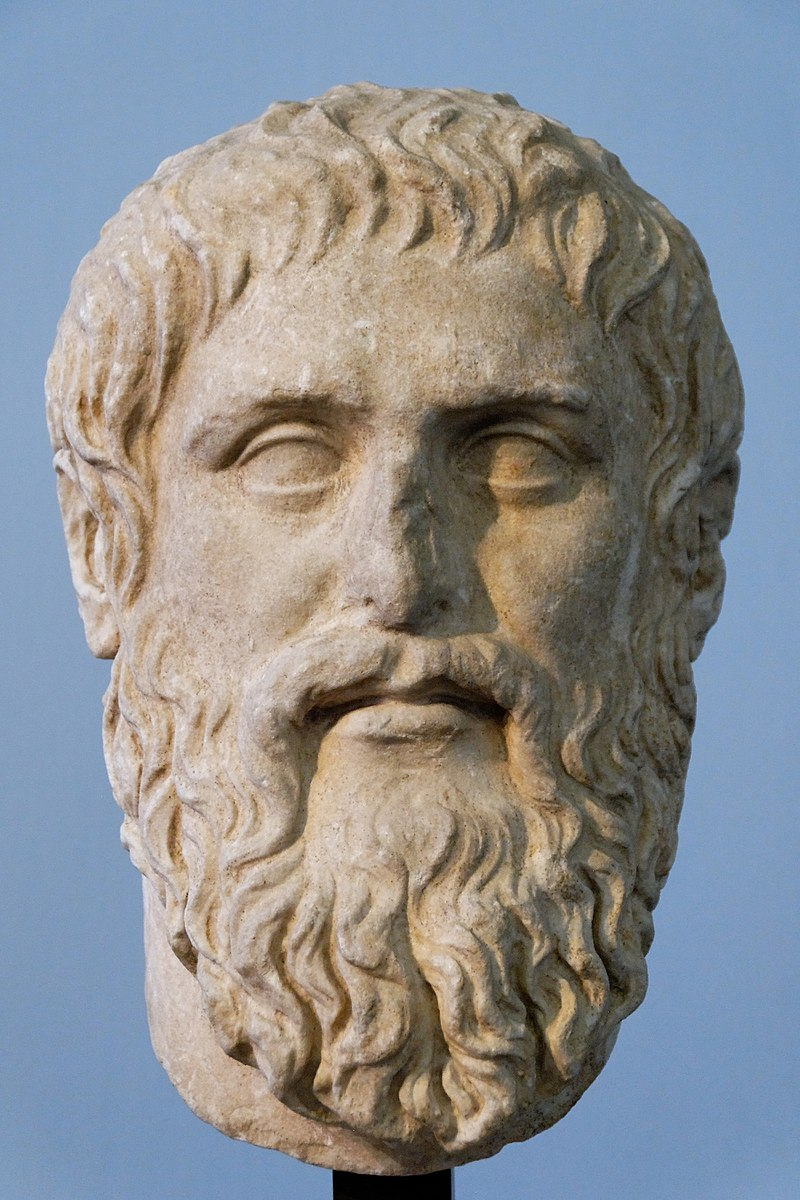
\includegraphics[width=1.5cm]{800px-Plato_Silanion_Musei_Capitolini_MC1377.jpg}
  \end{center}

  \begin{itemize}
  \item Objects exist ``out there'', independently of us.
  \item There is a universal notion of ``truth''.
    \begin{itemize}
    \item Every proposition is either true or false, even if \emph{we}
      can't see why.
    \end{itemize}
  \end{itemize}

  {\tiny
    \emph{Image: }By Copy of Silanion, Public Domain, \url{https://commons.wikimedia.org/w/index.php?curid=7831217}}
\end{frame}

\begin{frame}
  {``Intuitionism''}

  \begin{center}
    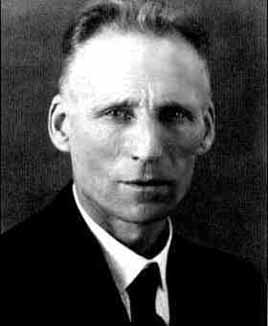
\includegraphics[width=1.5cm]{Luitzen_Egbertus_Jan_Brouwer.jpeg}
  \end{center}

  \sidenote{L.E.J. Brouwer, ~1900/10/20s}
  \begin{itemize}
  \item Objects exist as constructions within our heads.
  \item Including proofs of propositions
    \begin{itemize}
    \item We convince ourselves of the truth of a proposition by
      constructing evidence for it.
    \end{itemize}
  \end{itemize}

  {\tiny
  \emph{Image: }By Source (WP:NFCC\#4), Fair use, \url{https://en.wikipedia.org/w/index.php?curid=39567913}}
\end{frame}

\begin{frame}
  {Evidence based Interpretation}

  \sidenote{Instead of saying $P \mathop\Box Q$ is true when...}
  \begin{displaymath}
    \begin{array}{cl}
      \textrm{Evidence of...}&\textrm{is}\\
      \hline
      \true &\textrm{there always evidence of $\true$} \\
      \false&\textrm{there is no evidence of $\false$} \\
      P \land Q&\textrm{evidence of $P$ and evidence of $Q$} \\
      P \lor Q &\textrm{evidence of $P$ or  evidence of $Q$} \\
      P \to Q  &\textrm{a process converting evidence of $P$ into evidence of $Q$}
    \end{array}
  \end{displaymath}
\end{frame}

\begin{frame}
  {Evidence for Negation}

  We define $\lnot P = P \to \false$.
  \begin{itemize}
  \item evidence of $\lnot P$ is a process converting evidence of $P$ to evidence of $\false$
  \item but there is no evidence of $\false$
  \item so there can be no evidence of $P$.
  \end{itemize}
\end{frame}

\begin{frame}
  {Excluded Middle?}

  In two valued ($\true, \false$) logic, \emph{excluded middle} is valid for any $P$:
  \begin{displaymath}
    P \lor \lnot P
  \end{displaymath}
  The proof of validity (via truth tables) makes no commitment to
  which one is actually true.

  \pause
  \bigskip

  However, in terms of evidence, we have to \emph{construct} either
  \begin{enumerate}
  \item evidence of $P$, or
  \item evidence of $\lnot P$.
  \end{enumerate}
  For an arbitrary proposition $P$, this seems unlikely.
\end{frame}

\begin{frame}
  {\textcolor{red}{Failure} of Excluded Middle}

  For instance, if $x$ is a real number (has an arbitrarily long
  decimal expansion), then, in terms of evidence
  \begin{displaymath}
    (x = 0) \lor \lnot (x = 0)
  \end{displaymath}
  asks us to determine whether $x$ is $0$.

  \medskip

  But there is no process to do this in finite time.\\
  \sidenote{Another example: does this Turing Machine halt?}
\end{frame}

\begin{frame}
  {Intuitionistic Logic}

  Intuitionistic Logic is the similar to ``Classical'' Logic, except
  that it does not include the Law of Excluded Middle $P \lor \lnot P$
  for all propositions $P$.

  \medskip

  \rhighlight{Note:} this does not mean that $\lnot (P \lor \lnot P)$ is
  provable. There may be some $P$s for which $P \lor \lnot P$ holds.\\
  \sidenote{For example, $(x = 0) \lor \lnot (x=0)$ when $x$ is an integer}
\end{frame}

\begin{frame}
  {Summary}

  \begin{itemize}
  \item The system was have so far is \emph{sound} but not \emph{complete}
  \item We can make it complete by adding a rule for \emph{excluded middle}:
    \begin{displaymath}
      P \lor \lnot P
    \end{displaymath}
  \item But should we? What does Logic mean?
  \end{itemize}
\end{frame}

\end{document}
